\documentclass[12pt]{article}\usepackage[]{graphicx}\usepackage[]{color}
% maxwidth is the original width if it is less than linewidth
% otherwise use linewidth (to make sure the graphics do not exceed the margin)

\usepackage{scrtime} % for \thistime (this package MUST be listed first!)
\usepackage[margin=1in]{geometry}
\usepackage[usenames,dvipsnames]{xcolor}
\definecolor{aqua}{RGB}{0, 128, 225}
\usepackage[colorlinks=true,citecolor=aqua,linkcolor=aqua,urlcolor=aqua,hypertexnames=false]{hyperref}
\usepackage{xspace}
\usepackage{tikz}
\usepackage{placeins} % \FloatBarrier
\usepackage{amsmath} % \text, \cases
\usepackage{enumerate} % fancier enumeration (e.g., a,b,c, ...)
\usepackage{ragged2e} % \RaggedRight
\usepackage{grffile} % \RaggedRight

%% cleveref package for convenient hyperrefercing/citing:
\usepackage[nameinlink,capitalize]{cleveref}
\crefname{equation}{Equation}{Equations}
\Crefname{equation}{Equation}{Equations}
\crefname{figure}{Figure}{Figures}
\Crefname{figure}{Figure}{Figures}
\crefname{section}{\S}{\SS}
\Crefname{section}{\S}{\SS}

%% line numbers
\usepackage{lineno}\renewcommand\thelinenumber{\color{gray}\arabic{linenumber}}

%% comments
\newcommand{\hidecomments}{\renewcommand{\comment}[3]{}}
\newcommand{\comment}[3]{\textcolor{#1}{\textbf{[#2: }\textit{#3}\textbf{]}}}
\newcommand{\david}[1]{\comment{magenta}{DE}{#1}}
\newcommand{\jd}[1]{\comment{blue}{JD}{#1}}
\newcommand{\ben}[1]{\comment{purple}{BB}{#1}}
\newcommand{\mike}[1]{\comment{orange}{ML}{#1}}

%% code
\newcommand{\code}[1]{{\tt #1}}

%% misc macros
\newcommand{\etal}{\textit{et al}.\xspace}
%% for referencing TeX macros:
\newcommand\ttbackslash{{\tt\char`\\}}
\newcommand{\macro}[1]{{\tt\ttbackslash#1}}
\newcommand{\term}[1]{{\bfseries\slshape#1}}
\newcommand{\thickredline}{{\color{red}\bigskip\begin{center}\linethickness{2mm}\line(1,0){250}\end{center}\bigskip}}

%% abbreviations
\newcommand{\ie}{\emph{i.e., }}
\newcommand{\eg}{\emph{e.g., }}
\newcommand{\etc}{\emph{etc.}\xspace}

%% notation
\newcommand{\emx}[1]{\ensuremath{#1}\xspace}
\newcommand{\R}{\emx{{\mathcal R}}}
\newcommand{\Rzero}{{\mathcal R}_0}
\newcommand{\Rt}{\emx{{\mathcal R}_t}}
\newcommand{\littler}{\emx{r}}
\newcommand{\littlerwt}{\emx{r_{WT}}}
\newcommand{\littlervoc}{\emx{r_{VOC}}}
\newcommand{\B}{\emx{\beta}}
\newcommand{\Bwt}{\emx{\beta_{WT}}}
\newcommand{\Bvoc}{\emx{\beta_{VOC}}}
\newcommand{\textsub}[2]{\emx{{#1}_{\textrm{\small #2}}}}
\newcommand{\pmob}{\textsub{p}{mob}}


%% settings
\date{\today\ @ \thistime}

\definecolor{fgcolor}{rgb}{0.345, 0.345, 0.345}
\newcommand{\hlnum}[1]{\textcolor[rgb]{0.686,0.059,0.569}{#1}}%
\newcommand{\hlstr}[1]{\textcolor[rgb]{0.192,0.494,0.8}{#1}}%
\newcommand{\hlcom}[1]{\textcolor[rgb]{0.678,0.584,0.686}{\textit{#1}}}%
\newcommand{\hlopt}[1]{\textcolor[rgb]{0,0,0}{#1}}%
\newcommand{\hlstd}[1]{\textcolor[rgb]{0.345,0.345,0.345}{#1}}%
\newcommand{\hlkwa}[1]{\textcolor[rgb]{0.161,0.373,0.58}{\textbf{#1}}}%
\newcommand{\hlkwb}[1]{\textcolor[rgb]{0.69,0.353,0.396}{#1}}%
\newcommand{\hlkwc}[1]{\textcolor[rgb]{0.333,0.667,0.333}{#1}}%
\newcommand{\hlkwd}[1]{\textcolor[rgb]{0.737,0.353,0.396}{\textbf{#1}}}%
\let\hlipl\hlkwb

\usepackage{framed}
\makeatletter
\newenvironment{kframe}{%
 \def\at@end@of@kframe{}%
 \ifinner\ifhmode%
  \def\at@end@of@kframe{\end{minipage}}%
  \begin{minipage}{\columnwidth}%
 \fi\fi%
 \def\FrameCommand##1{\hskip\@totalleftmargin \hskip-\fboxsep
 \colorbox{shadecolor}{##1}\hskip-\fboxsep
     % There is no \\@totalrightmargin, so:
     \hskip-\linewidth \hskip-\@totalleftmargin \hskip\columnwidth}%
 \MakeFramed {\advance\hsize-\width
   \@totalleftmargin\z@ \linewidth\hsize
   \@setminipage}}%
 {\par\unskip\endMakeFramed%
 \at@end@of@kframe}
\makeatother

\makeatletter
\def\maxwidth{ %
  \ifdim\Gin@nat@width>\linewidth
    \linewidth
  \else
    \Gin@nat@width
  \fi
}
\makeatother



\title{A compartmental model for epidemic parameter estimation and forecasting, with applications to SARS-CoV-2}

\author{Michael Li, Jonathan Dushoff, David J.\,D.\ Earn,\\
  Irena Papst, Benjamin M.\ Bolker\\
  McMaster University}

\begin{document}

\linenumbers
\maketitle

\begin{abstract}
Compartmental epidemiological models are widely used to understand, manage, and forecast the SARS-CoV-2 (COVID-19) pandemic. 
We introduce a new compartmental modeling framework that shares many characteristics with existing models, but includes a number of new and noteworthy features.
In particular, it includes a flexible structure based on the \emph{flow matrix} (the \emph{per capita} rates of transitions between compartments) that allows it to be used interchangeably for discrete or continuous time and for deterministic or discrete-state stochastic models; the capacity to set starting conditions based on the expected distribution of states during an exponential phase of the epidemic; automatic computation of $\R_0$ and the mean and dispersion of the generation interval for specified parameters; explicit structures incorporating the intensity of testing and delays between test administration and reporting; time-varying parameters based on breakpoints, spline bases, or external covariates such as cellphone-based mobility indices; and the ability to calibrate model parameters to multiple data streams such as case reports, hospitalization and ICU admission rates.
We demonstrate the model by calibrating it to multiple COVID-19 time series (positive tests, negative tests, hospitalizations, and deaths) for each of the Canadian provinces from 2020-02-27 to 2020-08-30.
We estimate epidemiological parameters, including the effective reproduction number $\R_t$ over the course of these early six months of the pandemic.
\end{abstract}

\david{Target journal?  Ideas: PLoS Comp Biol}
\ben{PLoS Comp Biol seems to be shooting very high for this.
  I'd be fine with PeerJ/PLoS ONE, but would be willing to try harder,
  e.g. some low-tier-but-not-terrible epi or modeling venue}

%%\vfill
%%\subsubsection*{Our group's COVID-19 research}
%% A brief summary, including publications by our group to date, is available at\\
%%\url{https://mac-theobio.github.io/covid-19/}.
%%\david{I updated Park et al 2020, which is now published in JRSI.  JD,
%%  please update that page with anything else you've published.}

%%\vfill

\tableofcontents

%%\vfill

%%\subsubsection*{\underline{Current date range for analysis}: \ \ date_range[1] -- date_range[2]}

%%\newpage

\section*{Overview}

[Writing notes here for now so that I can use \code{fref}. This is not part of the draft.]

\subsection*{May notes}

Next step is to decide what results to use and how to frame them. I feel that \fref{Ont_calibration_base_forecast} and \fref{Ont_calibration_testify_forecast} are the beginning of a framework that could drive things forward: we tried this and got that. Here are the limitations or concerns – repeat. The big question in my mind is what's a good number/choice of things to show. How far forward in time or complexity are we willing to go? \ben{For my part, not much! I really want to get this out as the \textbf{minimal} adequate product.}

Reading now, I feel like the Results could be edited to make the supporting cast (most of the other figures) feel more like supporting cast. 

If we edit the Results the way I want, I think they will feel thin, so that brings me back to the question: what can we add? \ben{My personal feeling is that we should let them be thin.  The forecasting is no longer interesting (I think); what may be worth highlighting are the novel modeling aspects (there are a few).}

For even broader framing: here's the stuff we did during the pandemic, some of the problems we encountered, and some of the things we learned. We are describing these lessons because they may be helpful to people in future new outbreaks. We should also find a way to talk about how the development of macpan laid the groundwork for the development of macpan2, and to mention that it is here and we will be writing papers about it. \ben{OK, but not more than a few sentences.}

\section{Introduction}

SARS-CoV-2, the etiological agent of coronavirus disease 2019 (COVID-19), has been circulating in Canada since at least January 2020 \cite{onpr_200125}.
Response to the worldwide pandemic \cite{Li+20,Fauc+20} has been guided to a substantial extent by mathematical modelling \cite{Flax+20}.

%% Virological testing and contact tracing have been conducted to varying
%% degrees in different jurisdictions\david{REFS}.  While testing is
%% imperative for surveillance, its value for control is less clear.
%% Agent-based simulations indicate that the combination of testing and
%% contact tracing can be very effective in mitigating spread of
%% SARS-CoV-2 \cite{Ng+20}.  Emerging research is demonstrating that
%% saliva-based tests, as opposed to naso-pharyngeal swabs for RT-qPCR,
%% may be more effective, cheaper, and viable for the public to
%% self-administer \cite{Will+20,Wyll+20}, potentially making very
%% large-scale, frequent testing possible.

Here, we present a compartmental framework that was developed over the course of the pandemic. 
It incorporates the standard epidemiological compartments required to model COVID-19 as well as compartments that track health-care utilization and COVID-induced
mortality. 
Case reporting can be modeled either as a time-delayed convolution of incidence or by enabling a factorial expansion of the model that accounts for the testing status of individuals \cite{Fris+20}. 
The model also allows for time-dependent variation in any rate parameter --- particularly the transmission rate --- and allows this variation to be indexed by external covariates such as cellphone-based mobility metrics, or to follow smooth (spline) curves over time. 
The same model structure can be run as an ordinary differential equation, a discrete-time deterministic model, or a discrete-time stochastic model.
Finally, the model can be used to
(1) simulate specific scenarios for planning purposes;
(2) calibrate parameters to match multiple input time series such as hospital admissions or occupancy, cases, or deaths; or
(3) forecast future epidemic dynamics on the basis of past calibration.

\section{Methods}

\subsection*{Compartmental structure}

The epidemiological structure of the model is based on a susceptible-exposed-infectious-removed (SEIR) model with additional compartments reflecting the biology of COVID-19 and the structure of the health-care system. 
The COVID-19-specific compartmental structure of the model resembles many other COVID-19 models \cite{childs2021impact, tuite2020mathematical, kainChopping2021} in separating infectious individuals into sub-compartments reflective of the epidemiology of COVID-19; it additionally adds compartments for hospitalized individuals in acute care or intensive care. 
All symptomatic individuals are presumed to have undergone a period of pre-symptomatic infectiousness (\code{p}). 
Infections can be asymptomatic (\code{a}), mildly or moderately symptomatic (\code{m}) or severely symptomatic (\code{s}); all individuals with severe symptoms go to the hospital (acute care or ICU), or die before reaching hospital (e.g., in long-term care facilities).
Some fraction \david{add parameter symbol in brackets} of individuals who go to the ICU die. Recovered individuals (\code{R}) are assumed to be immune.  
The model includes additional compartments that facilitate book-keeping: cumulative hospital admissions (\code{X}), individuals in acute care after discharge from ICU (\code{H2}), and cumulative deaths (\code{D}) (\cref{fig:flowchart}).
(The version of the model discussed here was developed and used before vaccines were available and introduction of variants of concern and reinfections, we have since expanded the model to include other relevant compartments.)

\david{It is weird that we do not have a table listing all the parameters of the model.
I guess that's why the symbol for the proportion in ICU who die was not given above.}

This version of the model assumes homogeneous mixing --- all classes of infectives contribute additively to the force of infection (the \emph{per capita} infection rate of susceptibles).
We assumed hospitalized individuals do not contribute to the force of infection. \mike{re-write this point nicely? it is a strong assumption.}  
We did add one feature to the model to account for heterogeneity in susceptibility in the population, which we typically imagine is driven by heterogeneity in exposure (e.g., front-line and essential workers will be infected earlier), but could also be influenced by genetic, immunological, or other factors.
A \emph{phenomenological heterogeneity} parameter \david{not ``factor''} $\zeta$, modifies the force of infection by a factor of $\left(S(t)/N\right)^\zeta$. Since $0 < S/N < 1$, a positive value of $\zeta$ will make the force of infection decrease as the remaining fraction susceptible decreases, capturing the fact that the most susceptible individuals tend to be infected first, after which
the average level of susceptibility in the remaining population decreases.\david{revised that last sentence, which I kept misreading} While modelers have considered the dynamics of epidemiological models incorporating incidence functions of this general form \cite{WilsWorc+45,Liu+87}, previous attempts to model phenomenological heterogeneity have used transmission proportional to an exponential function of prevalence (i.e., $S I/N \times e^{-(I/N)^n}$ where $n$ is a shape parameter) rather than using a power law \cite{Will+06,Gran+09}. \ben{JD please check that this makes sense/expand where necessary; check Dwyer? Williams et al 2006: ``To allow for heterogeneity in sexual behaviour and to fit the observed asymptotic prevalence of infection, the transmission parameter takes the value $\lambda_0$ at the start of the epidemic and declines exponentially at rate $\alpha$ times the prevalence of infection.'' Granich et al. say ``To allow for heterogeneity in sexual behaviour and for the observed steady state prevalence of HIV, we let the transmission decrease with the prevalence, P. If n=1, the decrease is exponential; if $n=\infty$, the decrease is a step function. Both have been used in previous models (5, 29).'' Granich et al. also cite \cite{williamsHIV2006} (their ref. 29), but I don't see a transmission model in there anywhere ...}

%\begin{figure}[ht!]
\begin{figure}
\includegraphics[width=\maxwidth]{figure/flow.chart.crop.pdf}
\caption{Flow chart for basic compartmental mechanistic transmission model. 
Compartments: \code{S} (susceptible), \code{E} (exposed), \code{Ia} (asymptomatic infection), \code{Ip} (presymptomatic infection), \code{Im} (mild/moderately symptomatic infection), \code{Is} (severely symptomatic infection), \code{H} (hospitalized [acute care]), \code{ICUs} (ICU with prognosis of survival), \code{ICUd} (ICU with prognosis of death), \code{H2} (acute care after ICU stay). 
Compartments denoted by rectangles are accumulators, primarily used in the condensation step to compute incidences: \code{R} (recovered), \code{D} (dead), \code{X} (accumulator for cumulative hospital admissions).
\ben{prettify this further, \textbf{or} steal something better from Irena?}}
\mike{steal from Darren's product paper, it is in it}
\label{fig:flowchart}
\end{figure}

%% \begin{figure}[ht!]
%% \definecolor{shadecolor}{rgb}{0.969, 0.969, 0.969}\color{fgcolor}
%% \includegraphics[width=\maxwidth]{figure/ratematrix.pdf}

%% \caption{Flow matrix for basic compartmental mechanistic transmission
%%   model.  Gray indicates non-zero flows: compartments as in
%%   \cref{fig:flowchart}.  \ben{do we want this? It's equivalent to
%%     the flowchart, could be used to show differences in magnitude (via shading)
%%   if we sorted out the details} \jd{I think we don't.}
%%   }
%% \label{fig:flowmatrix}
%% \end{figure}

Internally, the model is defined by a \emph{flow matrix} $\mathbf{M}$, the elements of which specify the \emph{per capita} rates at which individuals move from one compartment to another.
For the basic model, the only element of the flow matrix that needs to be recomputed at each time step is the incidence (flow from $S$ to $E$); all other rates are piecewise constant (they are adjusted instantaneously when policies change, for example).
%%
This set-up allows for considerable flexibility:
\begin{enumerate}
\item For a numerical differential equation solver, we need the time derivatives of each compartment. The absolute rates are computed by columnwise multiplication by the state vector $\mathbf s$ (${\mathbf F}_{ij} = \mathbf{M}_{ij} \mathbf{s}_j$).
The gradient is the difference between the total flows into (column sums of $\mathbf F$) and out of (row sums of $\mathbf F$) each compartment.
\item For a discrete-time model, we compute the vectors of outflows and inflows as above, but simply compute the new states as (original state + (inflow - outflow)$\Delta t$).
\item We can also use a discrete-time model with a \emph{hazard correction} 
  \david{Is there a published paper that uses this terminology?  or at least a paper
    we can cite that uses the idea?  I believe that using this to make a discrete-time
    model is discussed by Hoppensteadt in an old book that I could find.}
  to the flows to address the possibility that a state will go negative due to an overly large outflow. Instead of the total \emph{per capita} outflow of a compartment being equal to the sum of \emph{per capita} flow to each other compartment ($\textsub{f}{tot} = \sum_i {\mathbf M}_{ij}$), we let the total outflow be 
\begin{equation}\label{eq:hazard}
\textsub{f'}{tot} = 1-\exp(-\textsub{f}{tot} \Delta t) \,; 
\end{equation}
the individual flows are then adjusted by a factor of $\textsub{f'}{tot}/\textsub{f}{tot}$.  \david{Notation is not ideal here.  $\textsub{f}{tot}$ depends on $j$; perhaps $f_j$ would be better?  Why $f$?  Maybe
  $M_j$?  Also $f'$ conveys ``derivative''.  Perhaps $\tilde f$ would be better?}
This adjustment accounts for the effects of depletion during the course of a time step.
\item Finally, if we choose to run a fully stochastic simulation, the flow matrix $\mathbf M$ is what we need to sample the flows between compartments as Euler-multinomial deviates \cite{breto+09}, which take the hazard correction \eqref{eq:hazard} and use it to compute probabilities for draws from binomial or multinomial random deviates.
  \david{Maybe explicitly write the formula for the probabilities
  in terms of the hazard correction.}
\end{enumerate}

While the flow matrix description is convenient for most epidemiological dynamics, there are a few epidemiological processes that are more naturally captured by absolute rather than \emph{per capita} rates, for example (1) when intensities of public health interventions such as numbers of tests or vaccines administered are reported by public health agencies; or (2) in models incorporating births or immigration.
We have typically handled the former case by taking observed vaccination or testing rates and dividing them by current compartment sizes in order to set the relevant entries in the flow matrix; we have not yet tried to build models including inflows from outside the system (the latter case).\david{The phrasing ``not yet tried'' feels odd in a paper.  Not sure how to express this.  Maybe ``the version of the software described here does not include inflows from outside the system (the latter case).''}

We typically compute the model dynamics deterministically, as a discrete-time model with a hazard correction \eqref{eq:hazard} (option 3 above).  Once the trajectories are computed, we reduce the full state vector to a more convenient, collapsed state vector in a step we call \emph{condensation}, for example by summing all of the infectious compartments to a single $I$ state vector, or collapsing the different acute-care ($H$, $H2$) or ICU ($\textrm{ICU}_\textrm{s}$, $\textrm{ICU}_\textrm{d}$)
\david{We should be consistent wrt font used for compartments.  We
were using \macro{texttt} earlier.}
compartments.
As well as allowing us to visualize model results more conveniently, condensation also allows us to compare the simulated state vector to available data streams.
In addition to summing compartments, we can also compute incidences as time-lagged differences of accumulator compartments (for example, differencing accumulated deaths $D$ to derive a mortality rate) or perform more complicated operations such as convolution\david{maybe cite Goldstein et al 2009, PNAS}. 
Our main use of convolution is to convert incidence---the force of infection (FOI) multiplied by the number of susceptibles---to a case-reporting (CR) time series: 
\begin{linenomath*}
\begin{equation}\label{eq:CR}
\textrm{CR}(t) = \sum_i \phi(i) (\textrm{FOI}(t-i) S(t-i))\,,
\end{equation}
\end{linenomath*}
where we typically set $\phi(i)$ to be a Gamma distribution with
moments chosen to match empirical estimates of case-reporting delays.
\mike{Do we have/need a formula for FOI?}
\ben{how did we pick these values? 
Probably don't have a formal ref but some statement of what we used to guess that this was reasonable would be good ...}.
\jd{Another option here would just be to say where $\phi$ is typically a Gamma distribution with moments chosen to match literature estimates>}
\ben{done, but still not clear that there are a lot of such estimates in the literature \ldots}\david{I added ``empirical'', which can cover unpublished estimates.}
When computing case reports from incidence we also assume a case-report proportion \code{c\_prop} to account for the fact that the majority of COVID infections are never reported \cite{Doug+2020}; this value is usually calibrated from data.

After condensation, the model also allows us to add observation error, which we typically simulate from a negative binomial distribution with a variable-specific dispersion parameter \cite{linden2011using}.

\subsection*{Expansion to accomodate testing}

At the cost of additional complexity, we can add explicit testing compartments to the model.  In the simpler version of the model, we assume that a specified fraction of infections are reported as cases (or we calibrate this fraction from joint data on cases and hospitalizations), and impose a distributed delay between infection and reporting via convolution \eqref{eq:CR}.
Here, we instead expand the susceptible and all infected compartments factorially to include the possibilities that individuals in those epidemiological classes have one of four testing statuses:
\begin{itemize}
\item untested;
\item tested and awaiting negative results;
\item tested and awaiting positive results; or 
\item tested positive.
\end{itemize}
After receiving negative results (whether true negatives, from individuals in $S$, or false negatives, from individuals in one of the infectious compartments), individuals cycle back to the untested sub-compartment where they can be tested again. After receiving positive results, they remain in the positively tested sub-compartment; depending on the model parameters, their transmission may be reduced due to self-isolation (controlled by the parameter \code{iso\_t}).  We assume here that people waiting for test results do not isolate.
Gharouni \emph{et al.}\/ \cite{Ghar+22} thoroughly analyze the epidemiological consequences of this structure in a simpler framework that expands a basic SIR model rather than the COVID-specific compartmental model (\cref{fig:flowchart}) as the foundation.
Individuals may progress between epidemiological compartments (e.g., becoming infectious or recovering) while awaiting the results of tests. In general, progressing individuals move to the same testing subcompartment, e.g., from \code{Im}-negative-waiting to \code{R}-negative-waiting.

We define a weight vector $w$ across epidemic compartments that gives weight $w_\textrm{a}$ to asymptomatic classes (\code{S}, \code{E}, \code{Ia}, \code{Ip}, \code{R}) and 1 to symptomatic classes (i.e., all other classes).
If $W$ is the weighted sum of compartment occupancies $X_i$, i.e., 
\begin{equation}
W = \sum_i w_i X_i/N \,,
\end{equation}
then for a daily \emph{per capita} testing rate $\rho$ we might expect that the corresponding \emph{per capita} testing rate in compartment $i$ would be ${\mathcal T}_i = \rho w_i/W$. 
\david{We should try to keep notation consistent with \cite{Ghar+22}.  I changed
$T_i$ to ${\mathcal T}_i$.  Not sure that's sufficient.}
However, under some extreme conditions (if testing is so extreme that few untested symptomatic people are left) this formulation can allow the \emph{per capita} testing rate to explode. To mitigate this problem we add a maximum daily \emph{per capita} testing rate $\tau$ to the model such that
\begin{equation}
{\mathcal T}_i = \frac{\rho \tau w_i}{\tau W + \rho} \,;
\end{equation}
see Appendix A.5 of \cite{Ghar+22} for details.  The testing flows out of each untested subcompartment are divided into flows to ``positive waiting'' and ``negative waiting'' compartments according to the infection status of the relevant compartment and specificity/sensitivity parameters (specificity/sensitivity refers to the probability that a truely negative/positive individual tests negative/positive).  \david{phrasing could probably be improved, but I felt we should define specificity and sensitivity} If tests are assumed to be perfectly specific and sensitive, then all individuals from non-infectious compartments (\code{S}, \code{E}, \code{R}) enter the ``negative waiting'' compartment and those from infectious compartments enter the ``positive waiting'' compartment.

We assume that all individuals admitted to the hospital for COVID-19 are immediately tested. (These tests are not included in the accounting of test distribution above, but in the COVID setting they represent a small fraction of the overall number of tests administered.)

\begin{figure}
  \includegraphics{figure/testFlow.1.Rout.pdf}
  \caption{Testing flow. Every epidemiological compartment is subdivided into the four subcompartments shown.
    Black arrows represent flows between subcompartments due to testing processes (test administration, reporting of tests); blue arrows represent progression between epidemiological compartments.
    Dashed arrows represent the accumulation of negative and positive test reports, which can be compared against data.
    \ben{is there a better version of this somewhere?}}
    \mike{what is the problem with the current figure?}
  \label{fig:testing_flow}
\end{figure}

\subsection*{Model parameterization}

The model allows for time-varying, piecewise-constant changes in any parameter. 
Our early analyses focused on changes in time-varying effective reproductive number (\Rt) due to behaviour change and non-pharmaceutical interventions, which we model by changing the transmission rate.
The transmission rate $\beta(t)$ is taken to be a time-varying function of the form $\beta_0 \beta_1(t)$ where $\beta_0$ is the baseline value for transmission from symptomatic individuals.
Individuals in different symptomatic classes (presymptomatic, asymptomatic, mild, severe) may have their transmission modified by a specified multiplier (given as model parameters); we assume that hospital transmission is negligible.
\david{Can we find a reference to support most transmission occuring in the community / outside hospitals?}
The time-varying (relative) transmission $\beta_1(t)$ can incorporate a variety of different effects, one at a time or in combination:
\begin{itemize}
\item abrupt (piecewise) changes on specified dates when control measures are known to have been implemented;
\item proportional to a power of observed mobility or some other exogenous proxy for contact behaviour:
\begin{equation}
  \beta_1(t) \propto \log(M(t))^{\pmob} \,, 
\end{equation}
where $M(t)$ is the relative mobility index at time $t$, for some power $\pmob>0$;
\item according to an arbitrary spline curve, i.e., a linear combination of components of a B-spline basis.
\end{itemize}
All of these sub-models for temporal change in the transmission rate can be subsumed under a single log-linear model:
\begin{equation}\label{eq:betamodel}
\log \beta(t) = \log \beta_0 + \XX\boldsymbol{c}
\,,
\end{equation}
where $\XX$ is a model matrix 
\david{not ideal that we have $X_i$ meaning something else entirely above}
that can contain any combination of covariates and $\boldsymbol{c}$ is a vector of covariates determining differences in the log of the relative transmission rate.
\david{Only $\boldsymbol{c}$ can vary in time, right?  We should therefore
write $\boldsymbol{c}(t)$ in \cref{eq:betamodel}.}
In particular, piecewise breaks correspond to indicator variables for which period an observation falls in; the mobility model corresponds to a column containing the log of relative mobility; and the spline model corresponds to a set of columns containing the basis vectors of a B-spline basis with specified knots.

In practice, when we use the model without incorporating covariates we adopt a simpler strategy of providing a list of the breakpoints and the parameters that change at those breakpoints --- a special case of the more general log-linear model. In the models illustrated below, we pick breakpoints to denote several time periods $\{P_1, P_2, \ldots\}$ and construct $\XX$ to allow the effects of mobility, and the baseline contact rate, to change at breakpoints.
Specifically, for each breakpoint we define a logistic transition curve 
\begin{equation}
S(j) = \frac{1}{1+e^{[t-t_\textrm{brk}(j)]/s}} \,,
\end{equation}
where $s$ (set to 3 days) defines the speed of transition. Because the baseline transmission rate is included in the model (as parameter \code{beta0}), we do not need to include an intercept in $\XX$; the first column is $\log(M(t))$, the dependence of (log) transmission rate on (log) mobility during the first period. For $j \ge 1$, subsequent columns $2j$ and $2j+1$ of $\XX$ are defined as $S(j)$ and $S(j) \log M(t)$, respectively. The parameters associated with these columns denote the change in baseline contact rate and the change in the effect of mobility between periods $j$ and $j+1$.
\ben{WZ: does this match what you think we did/your description below?}
  
\subsection*{Derived parameters and parameter setting}

It is useful to be able to compute several quantities derived from the parameters of a model, in particular:
\begin{enumerate}
\item the dominant eigenvector of the system in the exponential growth phase
  (as described below, we use this eigenvector to set sensible initial conditions for all state variables, including those that cannot be observed);
\item the basic reproduction number \Rzero and the intrinsic growth rate $r$;
\item the mean and coefficient of variation of the generation interval. 
\end{enumerate}
In principle we could compute these values directly from the flow matrix, by constructing the Jacobian matrix and the next-generation matrix and performing the appropriate eigenvector/eigenvalue calculations (as discussed by \cite{VandWatm02} for differential equations and \cite{Casw00} for discrete-time systems). However, we found it simpler to derive these values by simulation.

To compute the eigenvector, we run a simulation where we set the outflow from the susceptible compartment to zero (while maintaining the \emph{inflow} from $S$ to $E$), which mimics the dynamics near the disease-free equilibrium where susceptible depletion is negligible. After running the simulation for a long time (100 steps by default), the state vector is close to the eigenvector.  
We use this value to set starting conditions when starting near the beginning of the epidemic. 
It is easy to specify a scalar value (say, 1\% of the population) to indicate the initial size of the epidemic; by distributing these individuals according to the calculated eigenvector, we reduce numerical instability at the beginning of our simulations. 

To compute the other summaries (\Rzero, $r$, and moments of the generation interval) we rely on the fact that the software saves the force of infection at each time step. 
We simulate the progression of a \emph{single} individual through the infection process, i.e., setting the population size to 1 and setting the initial state to $E=1$ with all other compartments empty. 
Simulating deterministically then generates a time course of the probability that an individual is in any given box at a particular age of infection, and thus also the expected force of infection generated by a single infectious individual, as a function of time since infection. 
This vector $K(t)$ is the same as the transmission kernel in a renewal equation \cite{Cham+18}. 
We can easily compute 
\begin{equation}\label{eq:Rzero}
\Rzero = \sum_t K(t) \,, 
\end{equation}
mean generation interval  
\begin{equation}\label{eq:Gbar}
\bar G = \sum_t \frac{t\,K(t)}{\Rzero} \,, 
\end{equation}
and generation interval coefficient of variation,
\begin{equation}\label{eq:GCV}
\textrm{CV}(G) = \frac{\sqrt{\frac{1}{\Rzero}\sum_t K(t) (t- \bar G)^2}}{\bar G} \,.
\end{equation}
The growth rate can be computed by numerically solving for $r$ in the Euler-Lotka equation,
\begin{equation}\label{eq:Euler-Lotka}
\sum_t  K(t) e^{-r t} = 1 \,.
\end{equation}

\jd{Suggest dropping the detailed equations for Gbar and CV, but instead adding $g(t)$ and saying that we also calculate its mean and CV.}
\jd{Suggested easy ref is ChamDush15: http://dx.doi.org/10.1098/rspb.2015.2026 (instead of current Cham18)}
\ben{JD: please go ahead and implement this change}

In addition to its use in summarizing a given set of parameters, the computation of $\Rzero$, $r$, and the generation interval is useful as an initial step in calibrating the model. 
Estimates of these summary statistics are more broadly available \cite{park2020reconciling}, and more epidemiologically relevant, than the more specific mechanistic parameters describing the relative infectiousness and duration of each of the different infectious compartments (although this detailed information is still important for determining the effectiveness of interventions like contact tracing). 
We typically start with mechanistic parameters gathered from the literature and pre-calibrate them to specified target values of $r$ (which is easy to estimate from the observed initial growth rate of the epidemic in a region) and the mean generation interval by adjusting $\beta_0$ (baseline transmission) and simultaneously scaling the values of all of the epidemiological transition rates ($\sigma$, \textsub{\gamma}{s}, \textsub{\gamma}{m}, \textsub{\gamma}{a};
see \cref{tab:litparm})
by a single factor until the target values are achieved.

\subsubsection*{Calibration}

Once we have run a deterministic model simulation for a particular set of parameters (including a starting number infected, distributed across non-susceptible classes according to the exponential-phase eigenvector computed as described above) and we have some set of time series data to calibrate against (for example, case reports and hospital admissions), we can calculate a log-likelihood (e.g., \cite{Bolk08}). 
We assume that every observation is independently negative binomially distributed, with a series-specific estimated dispersion parameter (i.e., the variability in cases, hospital admissions, \emph{etc.}, will differ). 
We use standard nonlinear optimization algorithms built into R, such as Nelder-Mead, to find the maximum likelihood estimates; when we have had difficulty with numerical instability, we have performed an initial fit with differential evolution \cite{Mull+11} followed by a final fit with Nelder-Mead.

A link function can be added for any parameter in the model to constrain it to a sensible domain; the user specifies this by adding an appropriate prefix to the name of the parameter in the list of starting values for parameters to be calibrated. 
For example, specifying \code{log\_beta0 = -1} would specify that the baseline transmission parameter $\beta_0$ should be calibrated on the log scale, ensuring that the value of $\beta_0$ is always positive, and using a starting value of -1 on the log scale (i.e., initial $\beta_0 = \exp(-1)$). 
Specifying \code{logit\_nonhosp\_mort = -0.2} would specify that the value of \code{nonhosp\_mort} (the fraction of non-hospitalized mortality\david{is that the case fatality proportion outside hospital, or the proportion of deaths that occur outside hospital? I presume the former but it sounds like the latter}) should be fitted on a logit, or log-odds, scale, ensuring that it is bounded between 0 and 1, and using a starting value of $\beta_0 = \textrm{logit}^{-1}(-0.2) = 0.45$.

The model includes a general framework for adding a prior probability distribution for any parameter, using any distribution available in R. 
For example, \code{dbeta(nonhosp\_mort, 2, 2)} would specify a $\textrm{Beta}(2,2)$ prior for \code{nonhosp\_mort}.
We do not need to adopt a fully Bayesian framework to make use of priors; instead, we can think of them as convenient regularizing factors to keep the model-fitting process numerically stable. If we do want to be Bayesian, then the fitting procedure described above will return maximum \emph{a posteriori} (MAP) parameter values, not a sample from the full posterior distribution as is standard with frameworks that use Markov chain Monte Carlo.
\david{A standard ref is needed for MCMC.  \cite{Bolk08} or something else?}

For the province of Ontario, Canada, in 2020
we calibrated to deaths, and new confirmations, all of which were available publicly. 
In the expanded model, we can include time series of both positive and negative tests in our calibration. 
Reported new confirmations are the most reliable and voluminous source of epidemic information.
Unfortunately, they are also subject to many inherent biases, including substantial variation over time in \term{testing intensity} (\ie tests \emph{per capita} per day).

We simultaneously estimate the temporal pattern of the transmission rate [\cref{eq:betamodel}] (two mobility intercepts and three slopes), and several basic model parameters (\cref{tab:estparm}).
Other model parameters are taken from the literature (\cref{tab:litparm}).

\begin{table}
  \centering
  \input{litparm_table.tex}
  \label{tab:litparm}
\end{table}

We do not include hospitalization and ICU occupancy in our calibration because our model assumes all severe cases go through ICU, whereas during the early pandemic period
that we focus on here, many severe cases actually occurred entirely in Long Term Care Facilities (LTCFs); thus,
our model would not properly match the observed time series of hospitalization and ICU occupancy, or at least would fail to account for
severe cases outside of hospitals. Furthermore, capacity limitations in the health care system lead to ceilings on hospitalization that are
not represented in our model.
\ben{I think I got this statement right but am not sure: WZ/JD/DE, please check for correctness/clarity.}
\david{I removed ``properly'' since we make no attempt to represent capacity limits
  to my knowledge. What you describe accurately reflects our rationale in 2020, but we are currently happy to calibrate to hosp and ICU. Can we rephrase in a way
  that is consistent with us later deciding that fitting to hosp and ICU is OK?
  Is my additional phrase ``during the early pandemic period
that we focus on here'' a solution?}

\subsubsection*{Forecasting}

Our calibrations yield values for the parameters of our deterministic model (\cref{tab:estparm}).
Using the calibrated parameters and the estimated covariance matrix of the sampling distribution of the parameters, we draw many (typically 1000) sets of parameters from a multivariate normal distribution \cite{Bolk08,krinskyThree1991a} and feed them into the deterministic model to generate an ensemble of forecasts. We extend the end date of the calibration window (i.e., the last observed data point for calibration) to create a forecast window. In the forecast window, the user can either investigate scenarios by inputting covariates (i.e., relative mobility and/or testing rates, depending on the model) or assume that the last set of inputs remains constant through the forecasting window to obtain a
\emph{status quo} forecast.

\subsection{Data sources}

\subsubsection*{Public COVID-19 data for Ontario, Canada}

Daily reported data on COVID-19 testing and outcomes (confirmed cases, deaths, hospital and ICU occupancies) are publicly available for Ontario on the official provincal website:
\url{https://data.ontario.ca/dataset/f4f86e54-872d-43f8-8a86-3892fd3cb5e6/resource/ed270bb8-340b-41f9-a7c6-e8ef587e6d11/download/covidtesting.csv}.
However, this dataset does not include testing counts before 15 April 2020.  Since the beginning of the COVID-19 pandemic (and until the present at the time of writing), one of us (ML) has maintained a public web site containing Canadian COVID-19 data at the provincial level.  Data are frequently downloaded from a variety of sources and cleaned.  See \url{https://wzmli.github.io/COVID19-Canada/}.

\hypertarget{Mobility data}{}
\subsubsection*{Mobility data}

We use mobility data from Apple\footnote{\url{https://raw.githubusercontent.com/ActiveConclusion/COVID19_mobility/master/apple_reports/applemobilitytrends.csv}} and Google\footnote{\url{https://www.gstatic.com/covid19/mobility/Global_Mobility_Report.csv}}.  From these data we derive a \term{relative mobility index} using the ``driving'' index from Apple and the ``retail and recreation'' and ``workplaces'' indices from Google; we compute a 7-day moving average of these indices, rescale all of them to have a baseline (pre-pandemic) value of 1.0, and average the three indices (equally weighted), to obtain an overall index for each day.

\david{The ``important dates'' section is in \texttt{cuts.tex}.  Do we really not use those dates at all?}

\begin{figure}[ht!]
\includegraphics[width=\maxwidth]{figure/ontario_mobility.png}

\caption{Ontario mobility \ben{WZ: a previous version of this graph looked very different, with giant day-of-week effects.  The current version I'm seeing is much smoother ... do we know what happened/which was right?}}
\label{fig:Ont_mobility}
\end{figure}

\FloatBarrier

\hypertarget{sec:Results}{}
\section{Results}

\mike{Do we want to include some simulation to show the model works and can do the calibration?}
\david{I think that would strengthen the paper, if people have the strength for it.  While I'm always pushing for testing against simulations, I am most concerned about getting this paper finished and submitted soon.  If a fit to a simulation can be achieved quickly, then great.}

\mike{figure captions and make better plots}

\subsection{Base model}

Figure \ref{fig:Ont_calibration} shows the fit to data of a basic model\david{what is ``a basic model''?} that calibrates to COVID new cases and deaths for Ontario from 24 February 2020 (the first covid case reported in Ontario) to 30 August 2020.
This time frame captures the first wave of the COVID outbreak in Ontario. 
\mike{do we need a justification of the end date?}
\david{I moved the sentence about this being the first wave, but was
there really only one wave by end of of Aug 2020?}
The basic model was chosen to be the base model
\david{Huh?  Now we're assuming the reader understands the meaning
of ``basic model'' and ``base model'', neither of which have been defined.  I don't get this.}
because reported cases and death time series are most commonly applicable to public data \david{applicable to public data???  Is this supposed to mean that cases and deaths are what we can typically obtain publicly?}
for many juristrictions.
We did not explicitly include break dates (i.e., time-varying transmission rates) to match different public health measures and restrictions in place within the fitting window, the transmission rate is a function of time-varying intercepts and slopes on mobility index which is a sensible proxy for changes in behaviour responding to public health restrictions.\david{That was true in 2020 but is no longer true.
  We should rephase.  We could perhaps say ``was a good proxy\dots\ during the focal time period'' or something like that, but we then need to say this stopped being true eventually and some reference(s) to support this would be very helpful.}
Hospital occupancy and death on the other hand does not fit to the data well after the initial wave. This suggest the proportion hospitalized and death are lower and should be time varying as well. 

\david{The above paragraph is not clearly written.  It needs to be rewritten.  I'm not sure what was intended to be conveyed with various statements that I find unclear, so I'm just leaving this for now.}

\mike{keep only forecast plot?}

\begin{figure}[ht!]
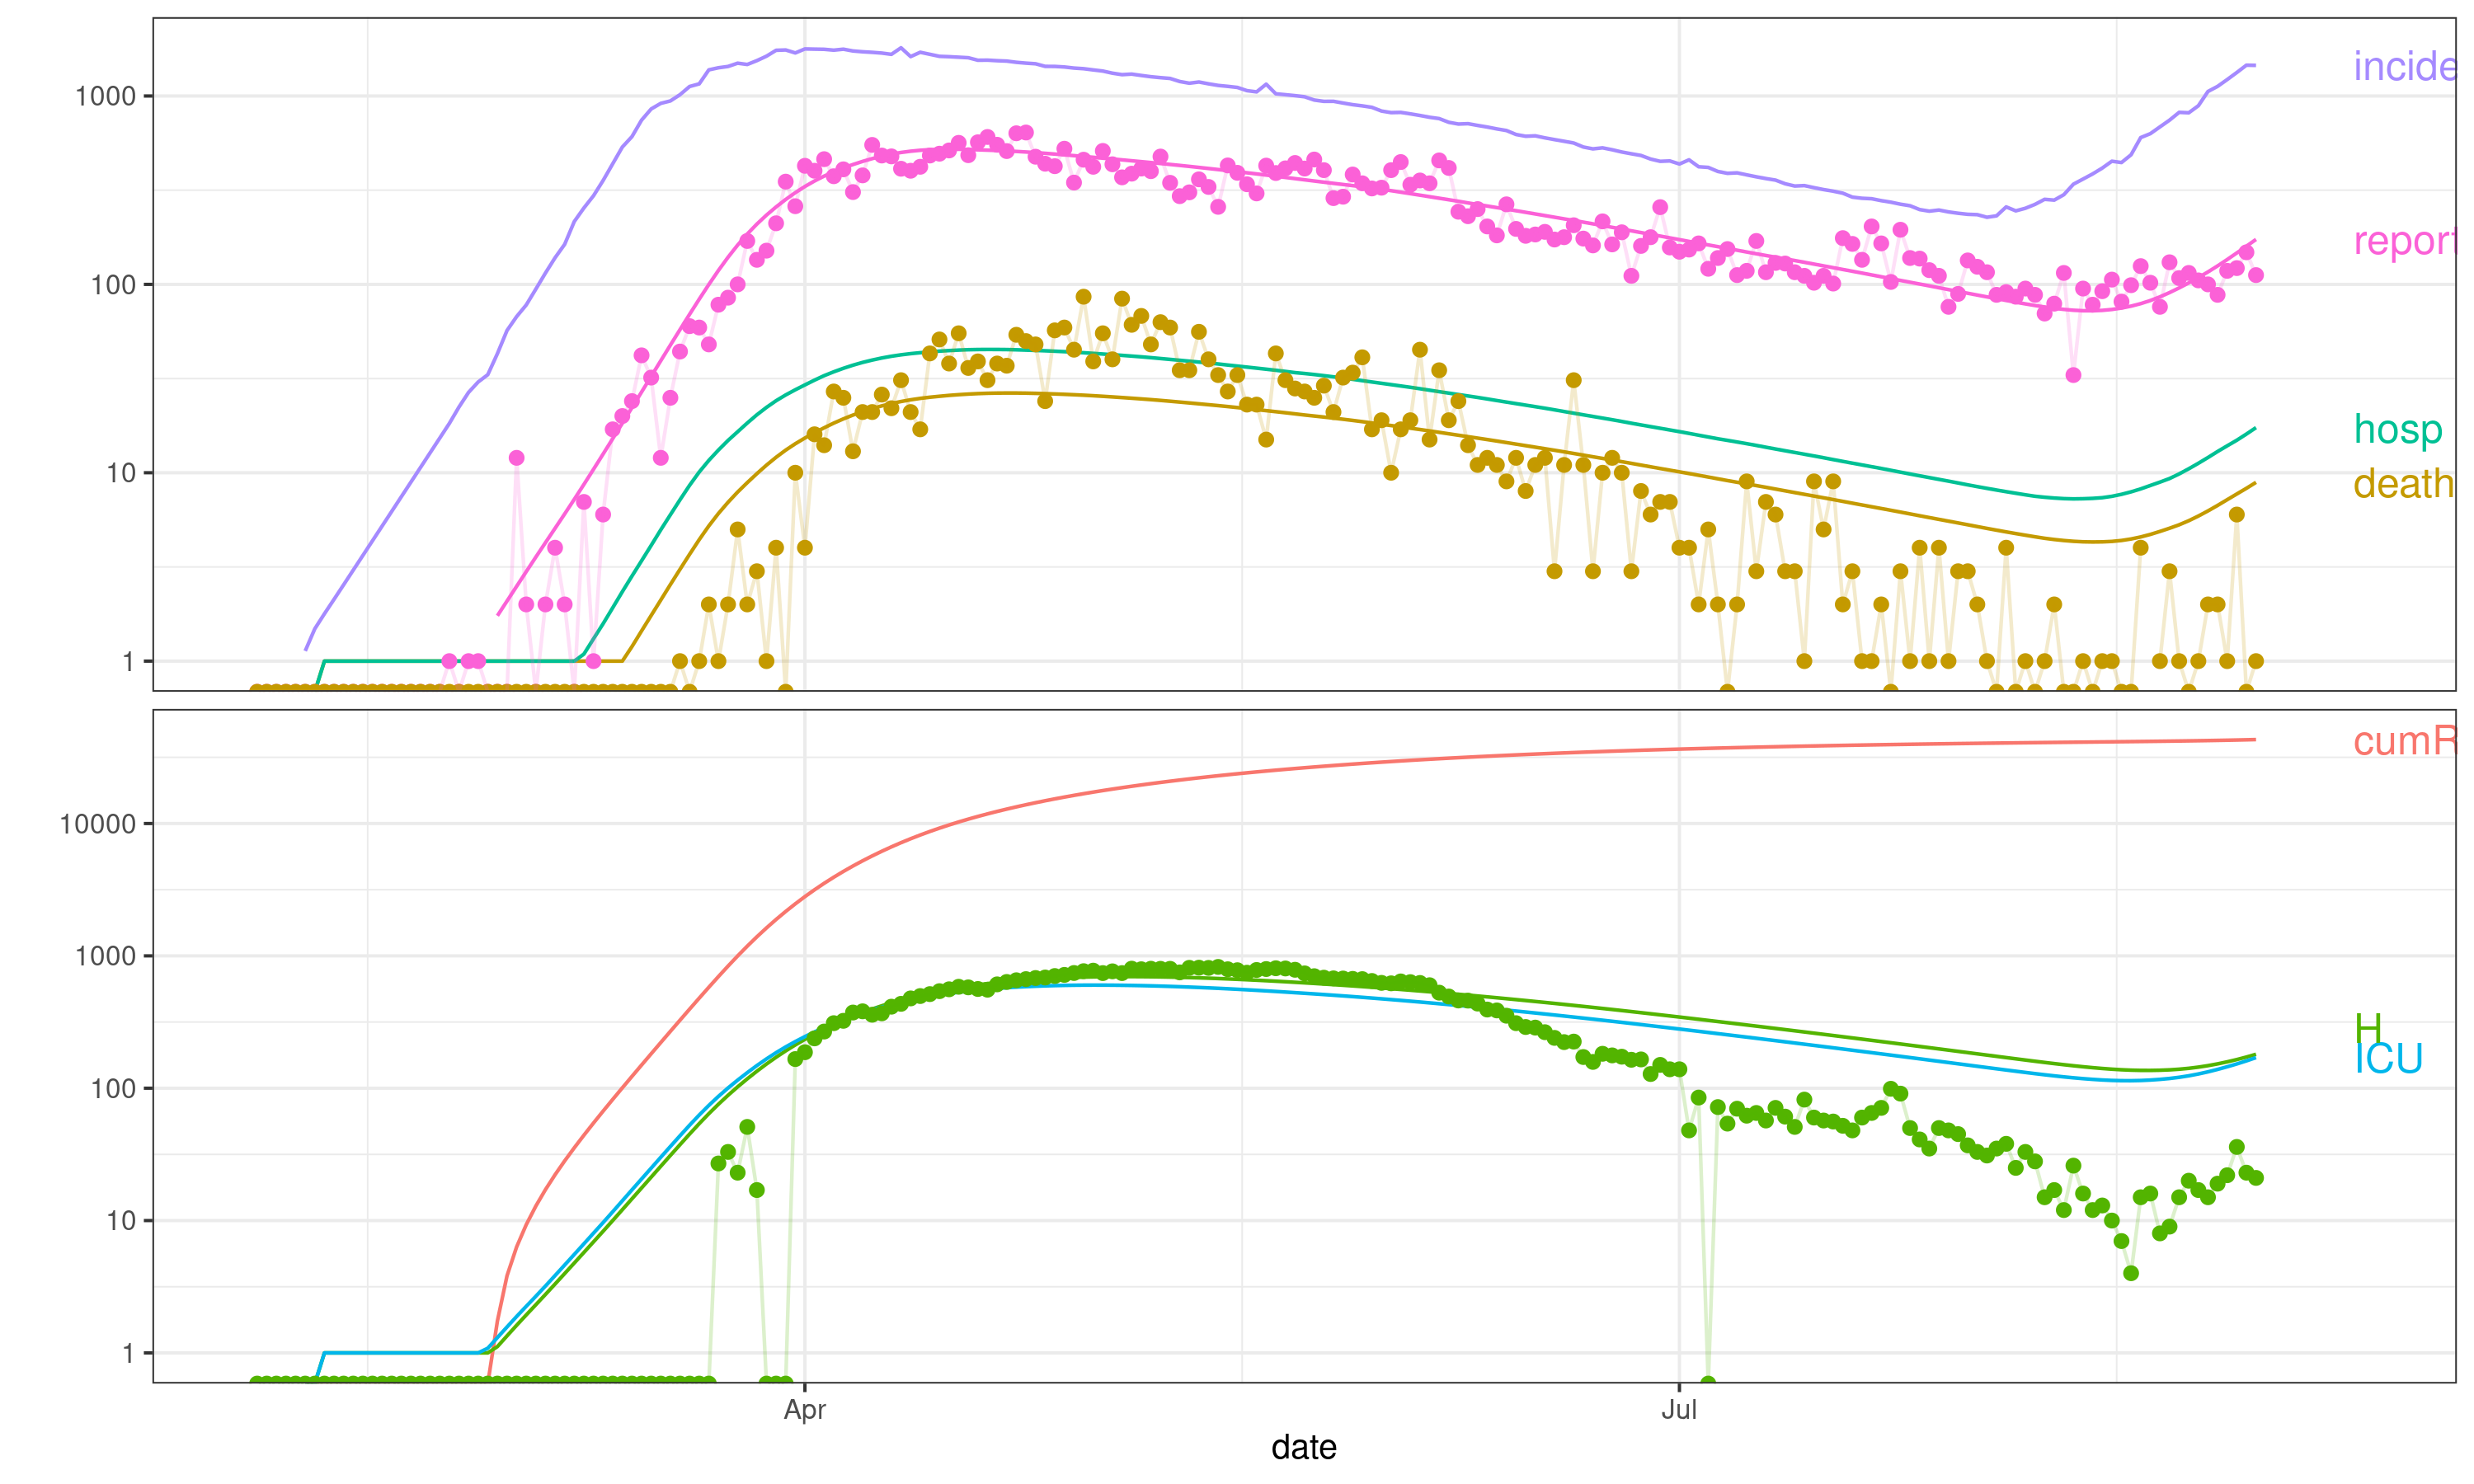
\includegraphics[width=\maxwidth]{figure/ontario_base.png}

\caption{Ontario calibration \ben{Take out incidence, cumRep? Mention that death and hospitalization rates declined (why?) and that we are only calibrating to reports/not allowing time-variation in hosp and mortality rates?}}
\label{fig:Ont_calibration}
\end{figure}

\begin{figure}[ht!]
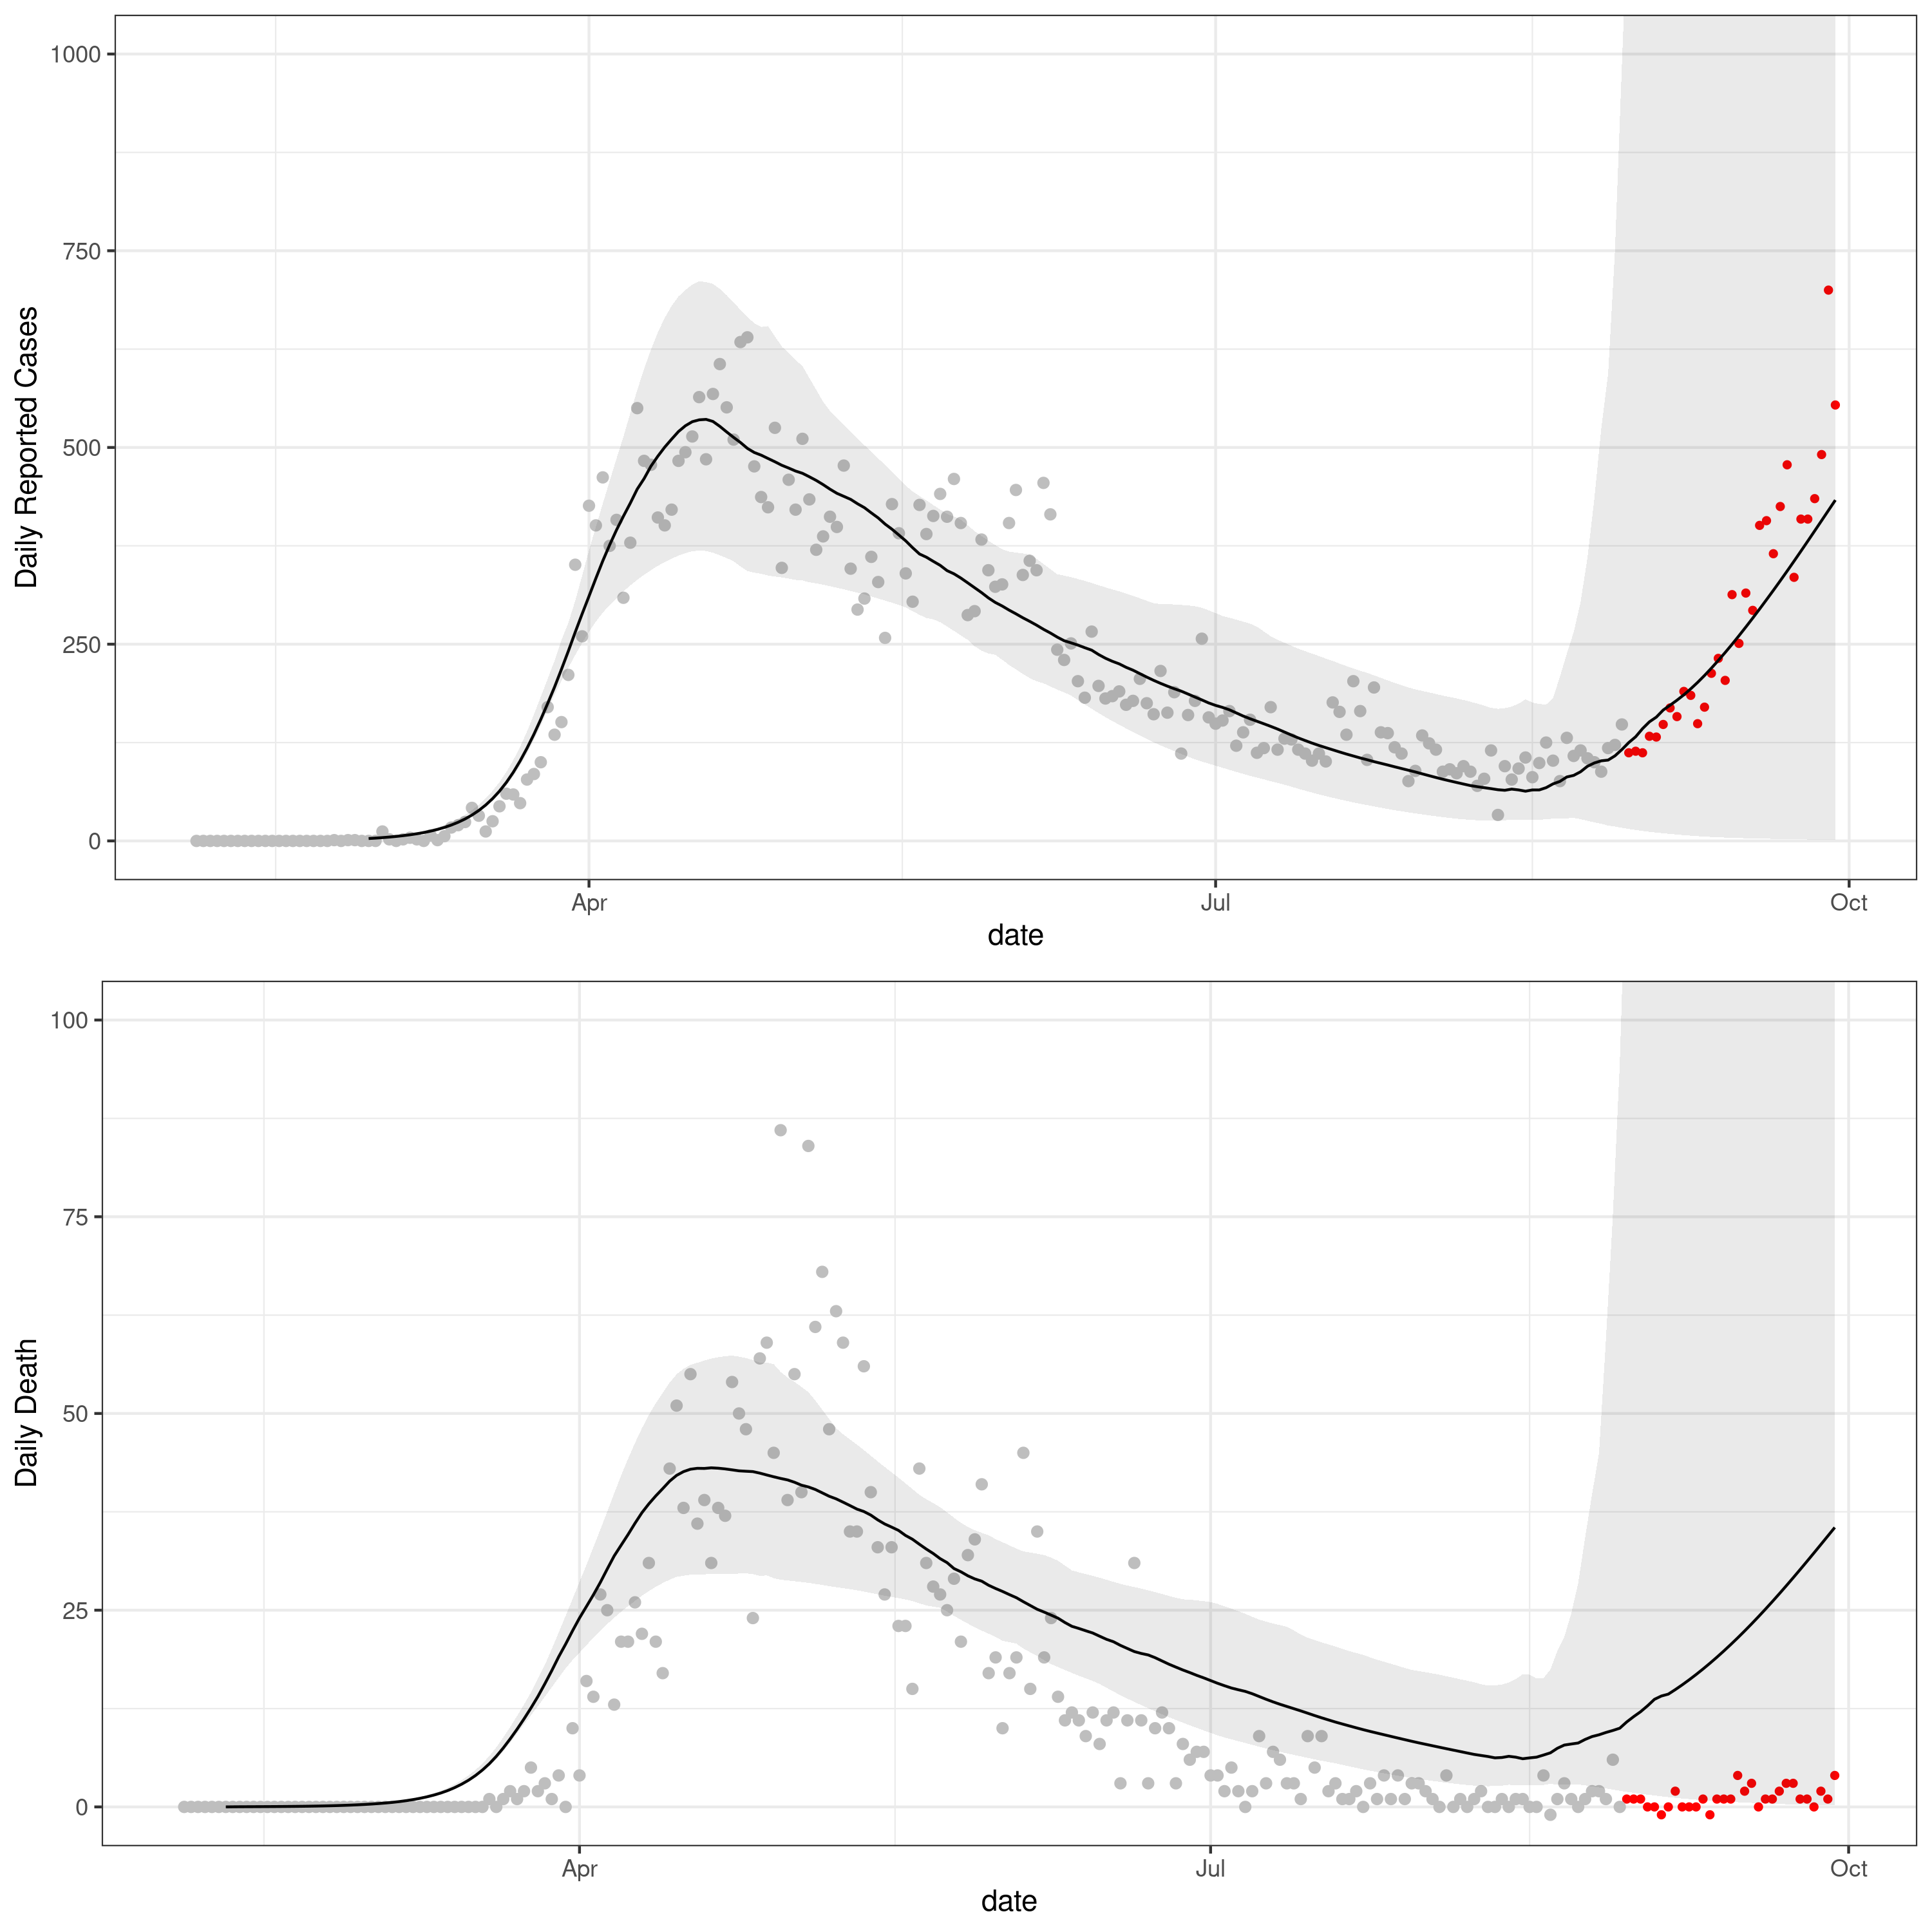
\includegraphics[width=\maxwidth]{figure/ontario_base_forecast.png}

\caption{Ontario base forecast. \ben{need to explain what's going on here; at the very least the caption should say (even if it's kind of obvious) that gray points represent calibration points, red are forecast points.  Why is the death forecast so far off?  Should we just leave it out (probably)? (WZ ...)}}
\jd{More comfortable leaving it out after we figure it out. It's bizarre. I could be convinced that it's water under the bridge, but it's worth a look.}
\label{fig:Ont_calibration_base_forecast}
\end{figure}

\begin{table}
\centering
\input{base_table.tex}
\caption{
  \label{tab:estparm}
  Parameter estimates for base model calibration. \ben{JD/DE: should some parameters (change in transmission etc.) be back-transformed? Are parameter names comprehensible?  Should we add confidence intervals/std errs? We should explain that dispersion model is converging to Poisson; do we need to justify/explain the very high value of $\zeta$ (phenom het)?}\david{We definitely need to comment on
    the value of $\zeta$; it seems absurdly high.}
  \david{CIs would be nice.}
}
\end{table}

\FloatBarrier

\subsection{Incorporating testing flows}

The base model is relatively simple but does not account for testing practices. Testing strategies changed frequently over the course of the pandemic due to availability of testing facilities and shifting regulations on eligibility for testing.

Figure \ref{fig:Ont_calibration_testify} shows the results from calibrating the model to positive tests, with the testing flow incorporated and with observed testing rates fed into the model as a known series.
The variation in the predicted line is driven by high-frequency changes in testing rate, including day-of-week effects.
It also shows the daily testing in Ontario in the calibration time frame. The vertical line is the cut-off between the calibration window (before September 1st 2020) and 30 days beyond it for the forecast window. The testing intensity over the forecast window is assumed to be constant at the last observed testing intensity on August 30th 2020 (since the actual increase in testing that occurred during the forecast window was not known at the time of the forecast).
\david{I suggest using open circles during the forecast window, as we do for observed cases and hospitalizations.}

\begin{figure}[ht!]
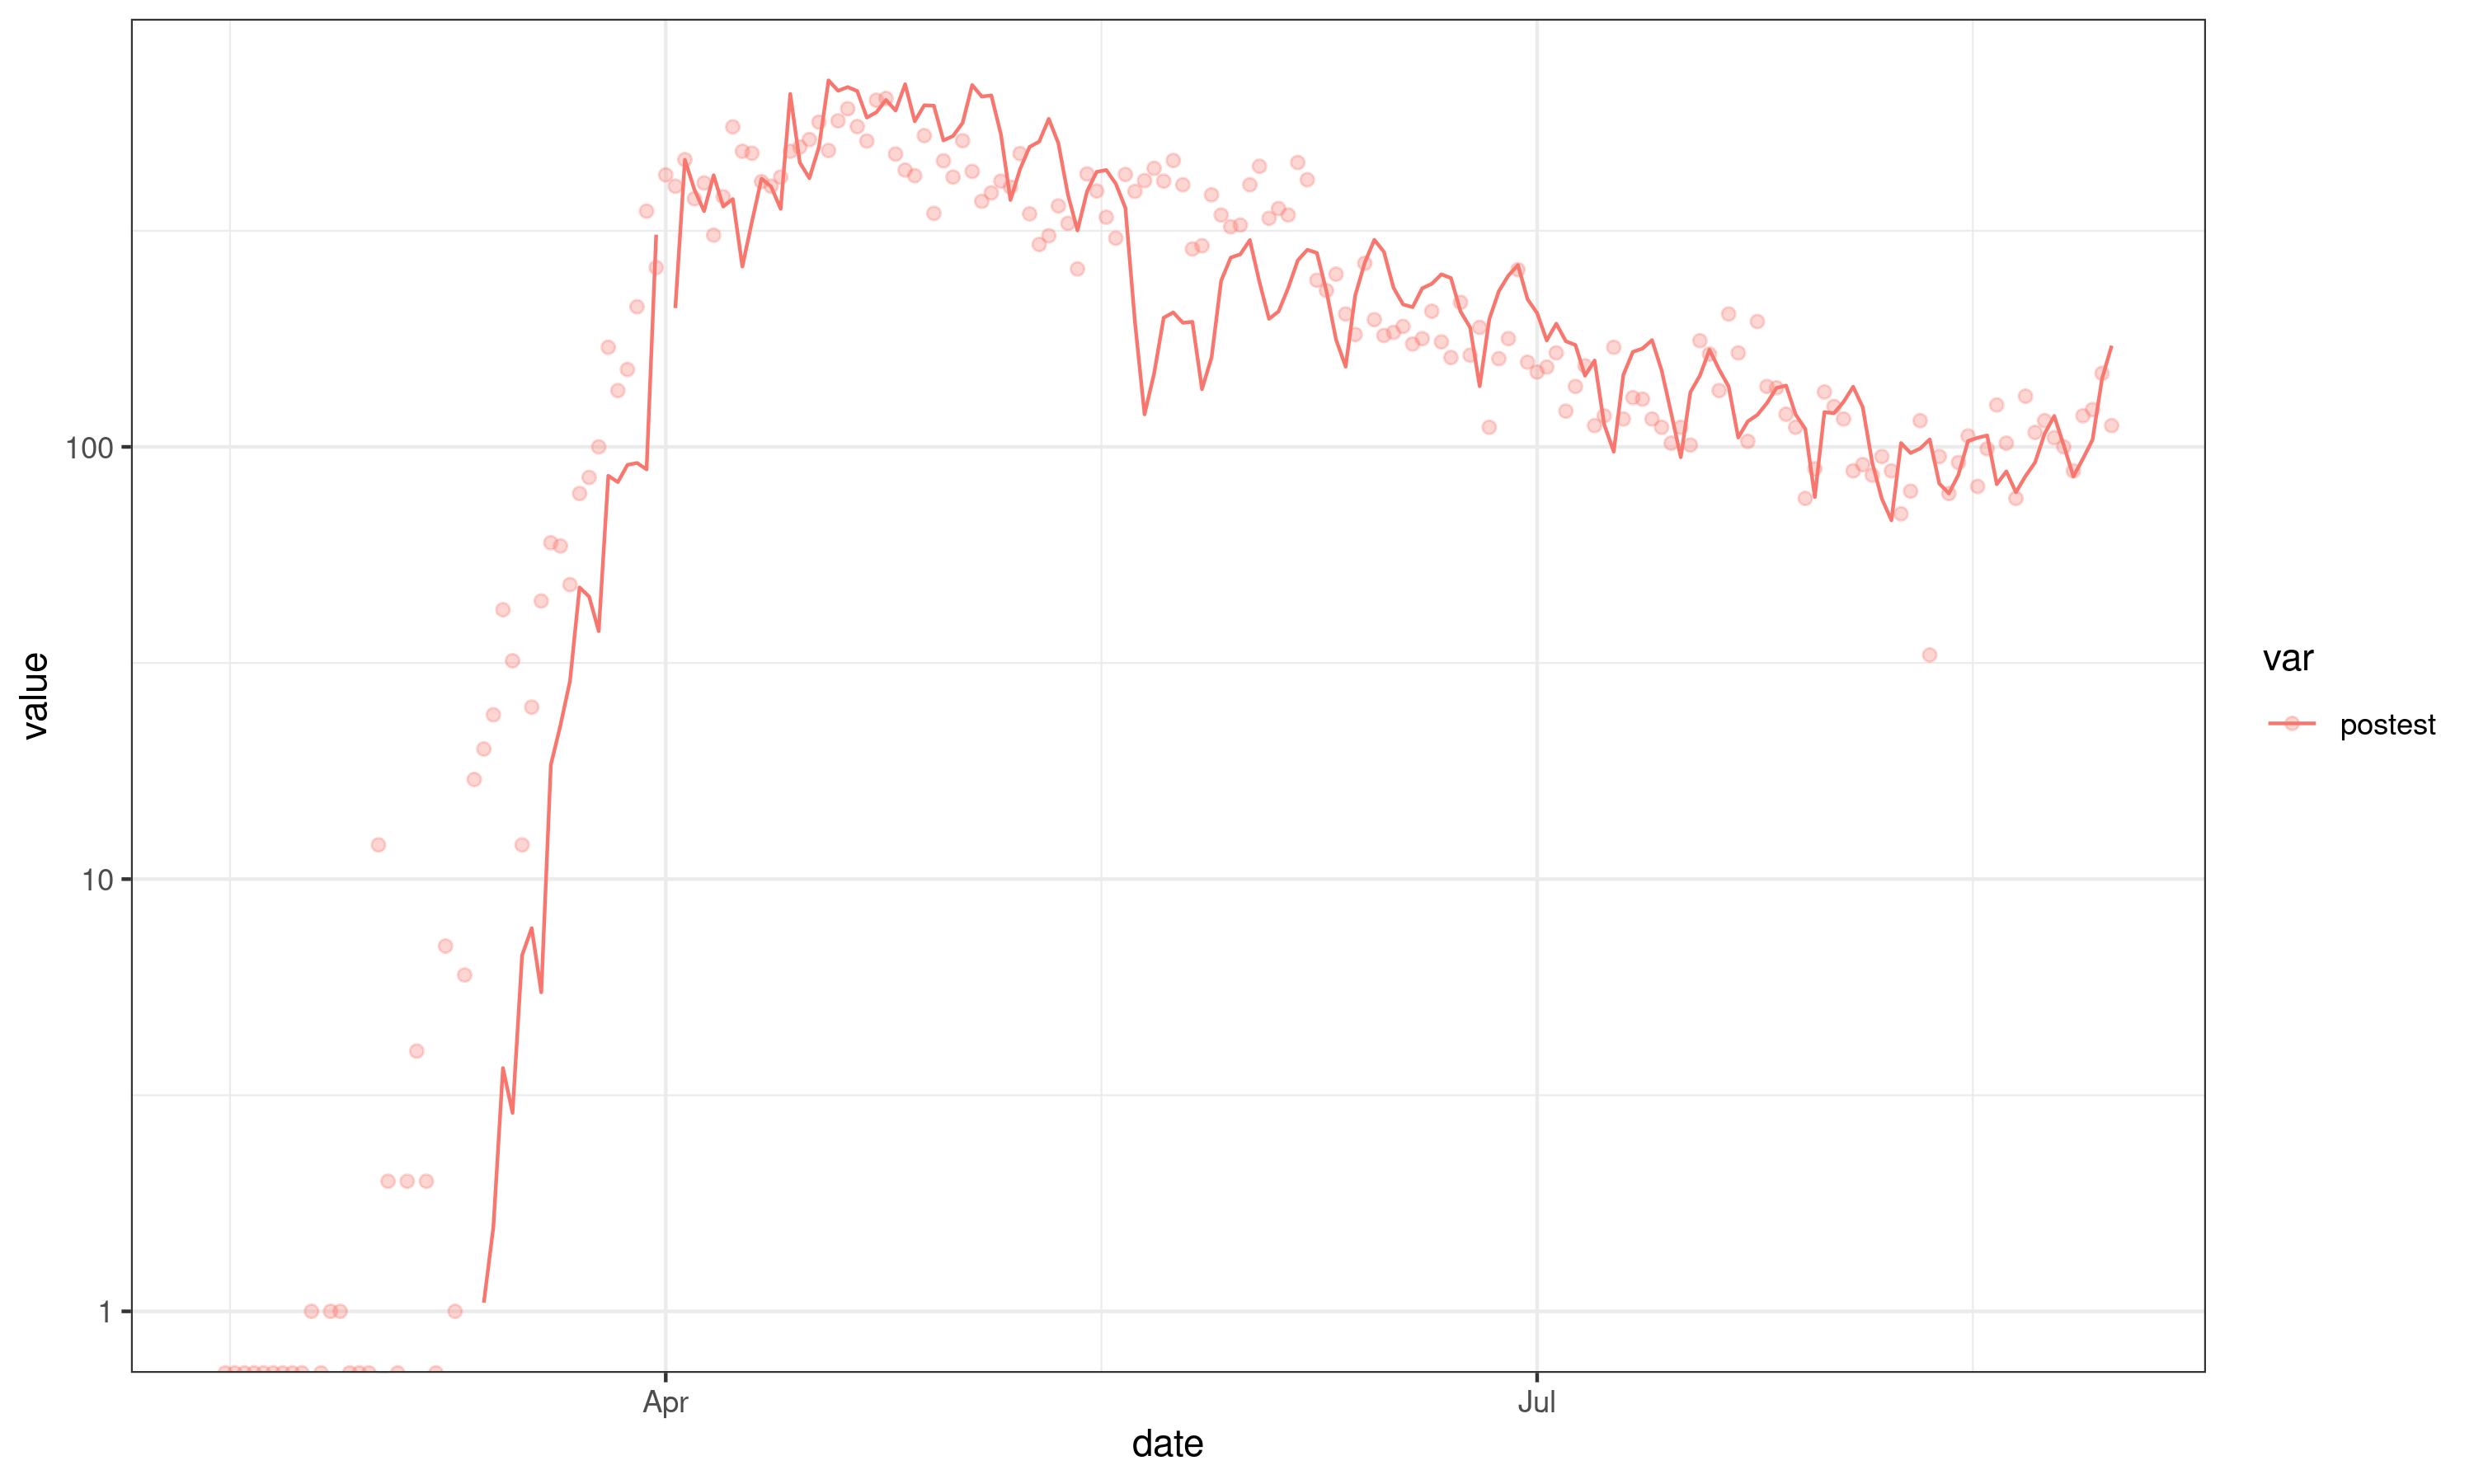
\includegraphics[width=\maxwidth]{figure/ontario_testify.png}

\caption{Calibration of positive tests and testing intensity}
\label{fig:Ont_calibration_testify}
\end{figure}

\begin{figure}[ht!]
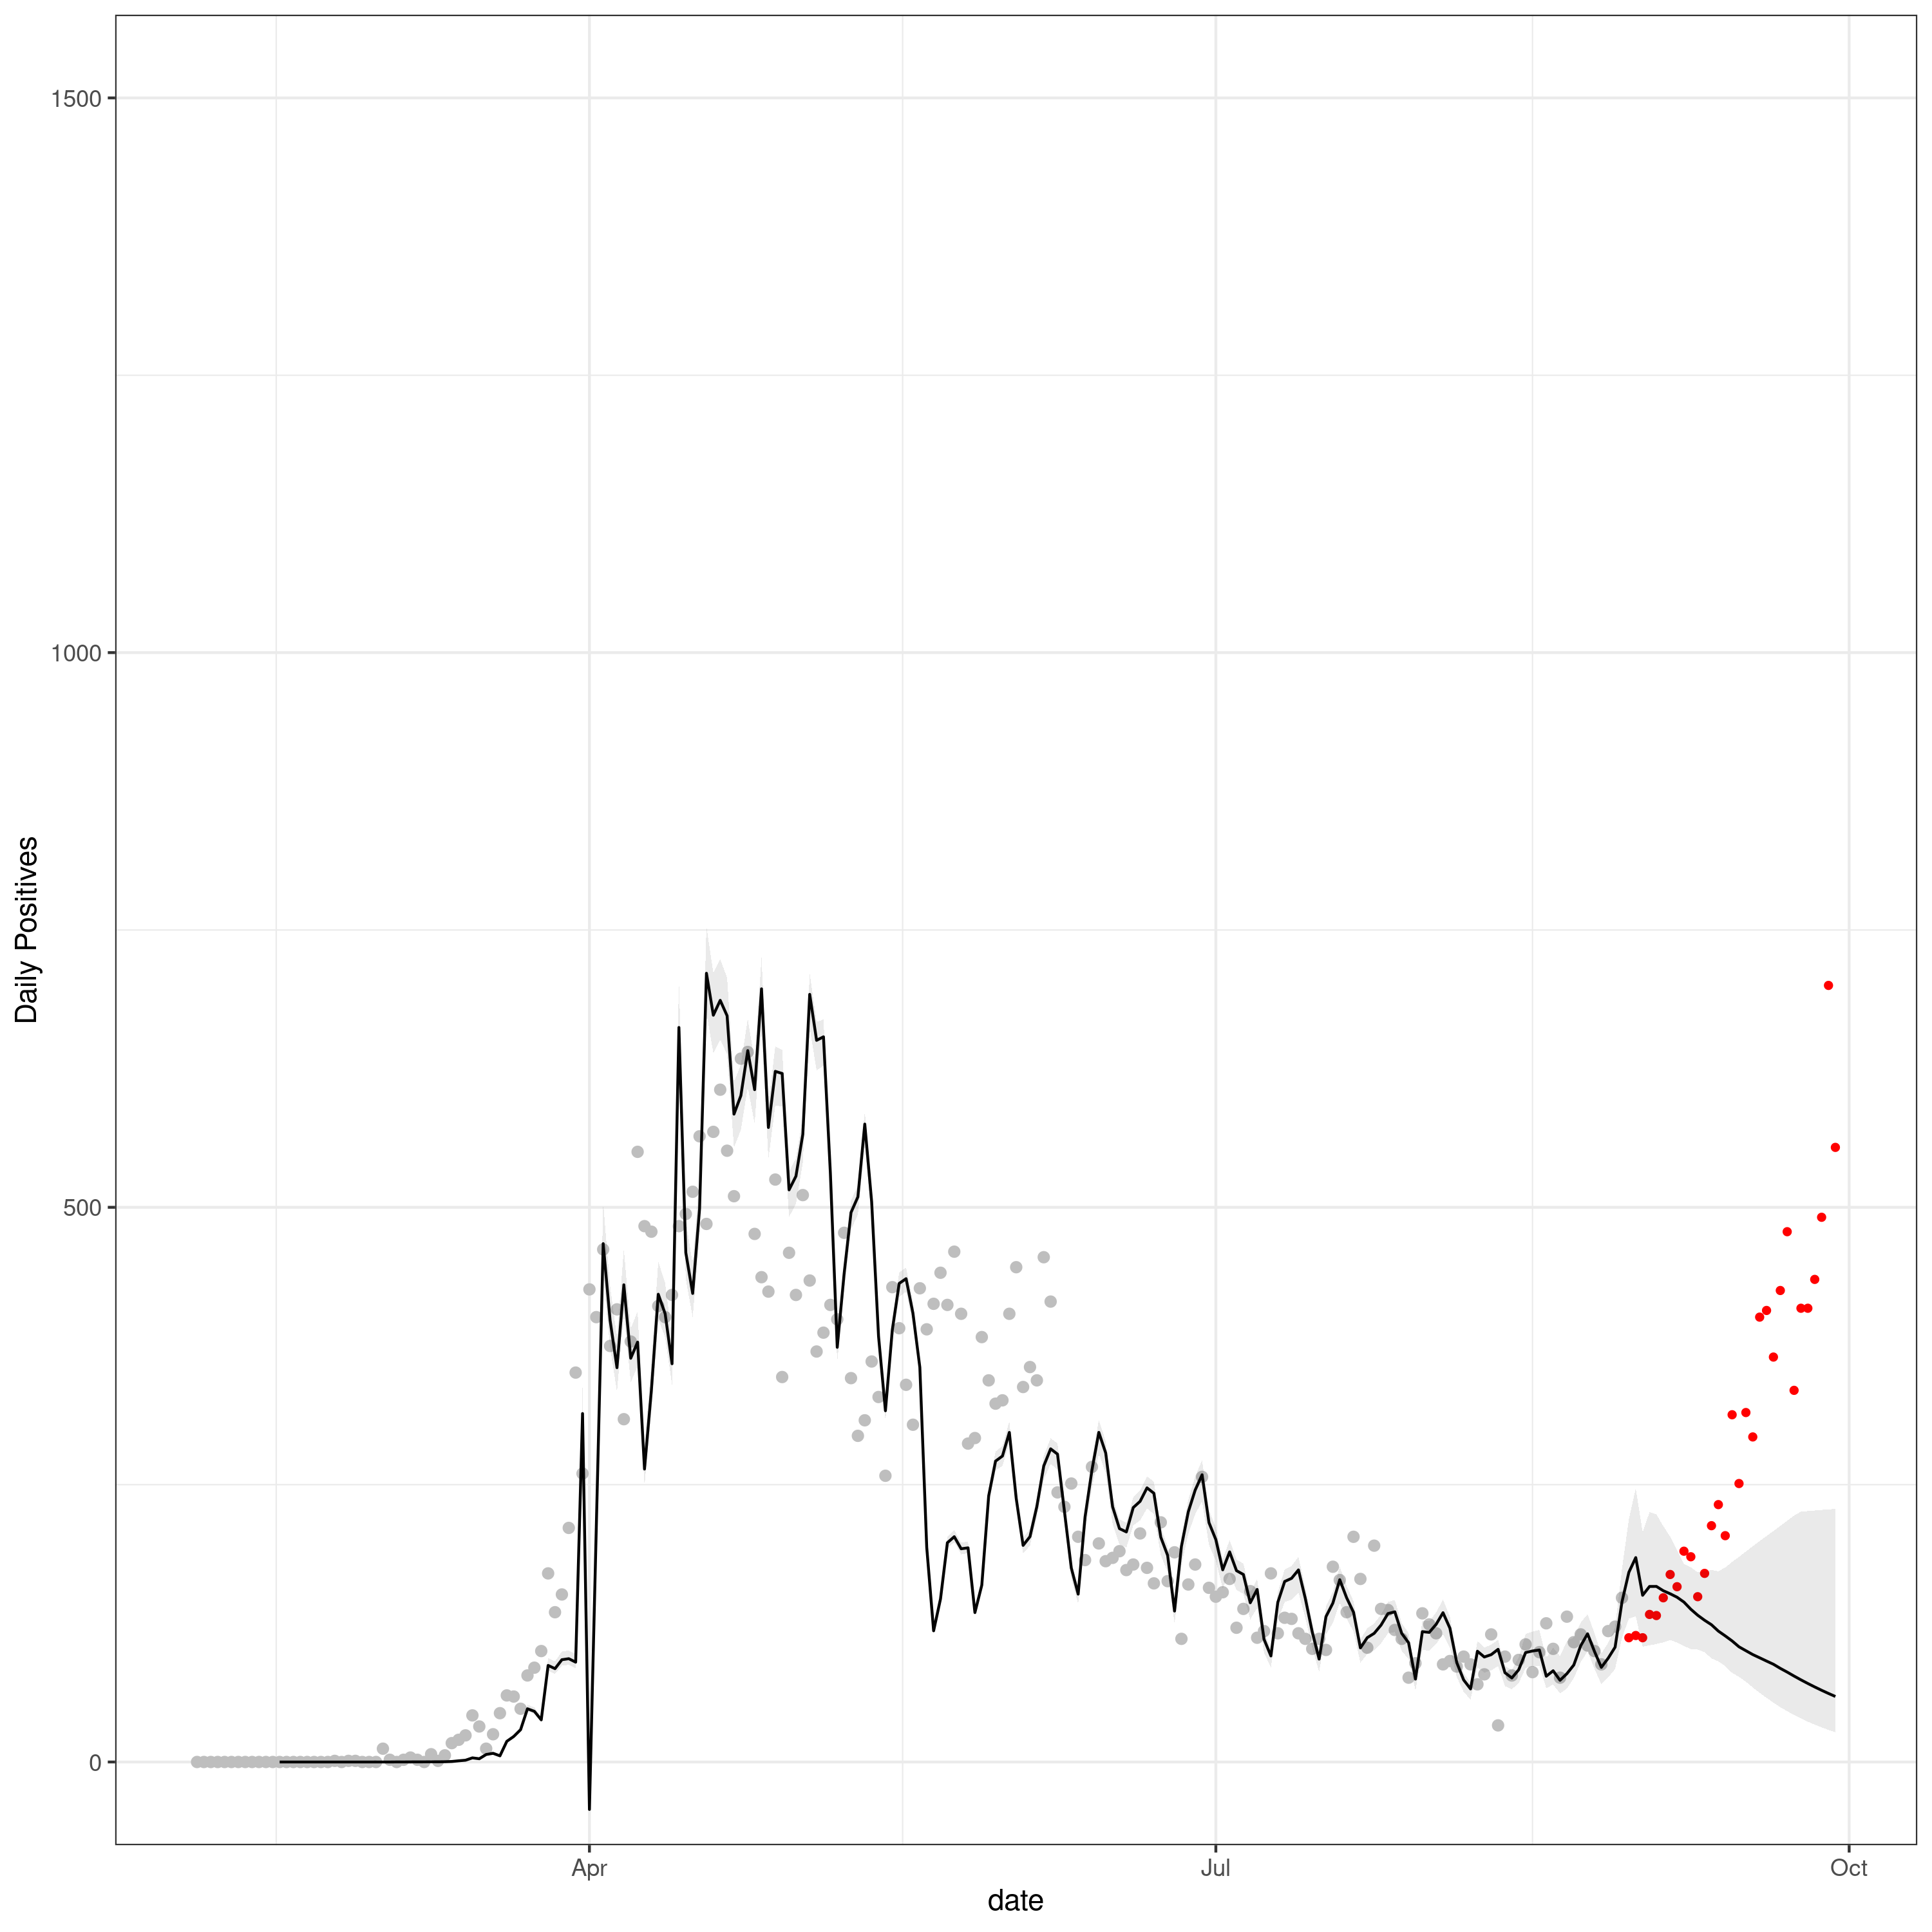
\includegraphics[width=\maxwidth]{figure/ontario_testify_forecast.png}

\caption{Ontario calibration with testing flows}
\label{fig:Ont_calibration_testify_forecast}
\end{figure}

\mike{We (I) probably should make another forecast using the testing intensity of the forecast window. Thoughts?}
\david{Yes it would be good to see how using the correct testing intensity affects the forecast.  This needs to be expressed carefully to avoid confusion.  We need to get across that this emphasizes how much better the forecast would be with advance knowledge of how testing intensity would change over the forecast period.}

\begin{table}
\centering
\input{testify_table.tex}
\caption{Parameter estimates for testify model calibration. \ben{Contrast with non-testify results.  Maybe instead of this table we can include a figure that shows the two values along with confidence intervals? (Have to be a little careful about the scaling - i.e., which parameters it makes sense to show on a common scale ...)}
\david{Can we explain the factor of 10 difference in $\zeta$?}}
\label{table:testify}

\end{table}

\FloatBarrier

\section{Discussion}

We have fitted two models that vary in complexity to SARS-CoV-2 daily reporting and death time series data for Ontario, Canada, from 1 March to 30 August 2020.  Our simple base model is typicalof compartmental epidemic models used to study infectious disease epidemics.  The testify model \david{The ``testify'' terminology has not been defined.  Do we want to define it and use it because we like the term? or should we just refer to the ``model with testing flows'' or something like that so referees don't think we're goofy?}  is a practical expansion of the base model that allows us to take advantage of data on time-varying testing practices and policies.

\subsection{Limitations}

Our model assumes homogeneous mixing of the population. 
No age-related or spatial contact structure is considered. 
\david{The following sentence needs to be rewritten.  I don't understand what was intended to be expressed.}
We did not include hospitalization in the calibrations due to reporting from capacity issues which became a serious issue with the admissions and occpuancy underreporting the severity of the pandemic.
In addition, long-term care facilities (LTCFs), where many elderly people in Canada have died without going to hospital, have not been modelled explicitly.  
While we do not anticipate any qualitative differences in results, explicitly creating compartments and calibrating to data for LTCFs would likely allow us to match ICU occupancy and forecast
pressure on ICUs more accurately but will not resolve the issues on hospital intensity.
\david{the last phrase needs to be rephrased.   What is ``hospital intensity''?}

\subsection{Conclusions}

\david{This conclusion paragraph leaves a lot to be desired.  I think we should discuss what we think the key take-home messages should be, and then write a new conclusion paragraph.  We should also state that we have continue to develop the software during the pandemic, and will describe further innovations in subsequent papers.}

SARS-CoV-2 continues to be a global burden after 3 years. 
Here we demonstrated a simple modeling framework that can flexibly fit epidemic data and easily allow additional complexities to account for features during the epidemic. 
We learned two things about fitting epidemic data. 
First, it is important to have ways to incorporate time-varying parameterizations fitting changes in the observed data or behavioural changes. Time-varying transmission rates played an important role in our calibration. 
Second, allowing for testing intensity to disaggregate the transmission rates through time (i.e. does increase in positive cases/confirmation due to an increase in transmission or testing capacity). 
The flexibility of incorporating various time-vary parameterizations allows users to make more realistic features and scenario exploration. 

\david{\macro{input\{nextsteps.tex\}} has been commented out.  There may be useful comments in there that would help with Discussion/Conclusions.}

\thickredline

\clearpage

\section{To do}

\begin{itemize}
\item find and clean up \code{estparmtab}/\code{litparmtab} (done)
\item clean up Tables 1 and 2 (WZ?)
\item should we include fits to simulations or not?
\item Clean up figures, improve captions  
\item Discussion and conclusions
\item output/include figs as PDF rather than PNG (JD, WZ?)
\item \david{In the original PHAC report, we showed fits to all
    the large provinces.  I'm OK with discussing Ontario only, but just checking that change was intentional.  I've move the commented-out appendix to \texttt{cuts.tex}.}
\end{itemize}

\clearpage

\bibliographystyle{vancouver}
\bibliography{McMasterReport}

\end{document}
